%\section{稳态传导方程的有限体积法}
\subsection{一维稳态传导问题}
\begin{frame}{一维稳态传导问题}
某一运动要素$\phi$的一维稳态传导问题:
\begin{equation*}
  \frac{\mathrm{d}}{\mathrm{d} x}(\Gamma \frac{\mathrm{d} \phi}{\mathrm{d} x}) +
  S = 0
\end{equation*}
其中,$\Gamma$为传导系数,$S$为源项。在边界点上$\phi$的值给定。
\end{frame}

\subsection{步骤一:网格生成}
\begin{frame}{网格生成}
  \begin{itemize}
    \item 将计算区域划分为互不重叠的离散控制体
    \item 在A和B之间均匀的布置一系列的节点
    \item 每个控制体的边界位于相邻节点的中线处
    \item 在计算域边界处设置控制体是比较常见的做法
  \end{itemize}
  \vspace{1cm}
\begin{center}
  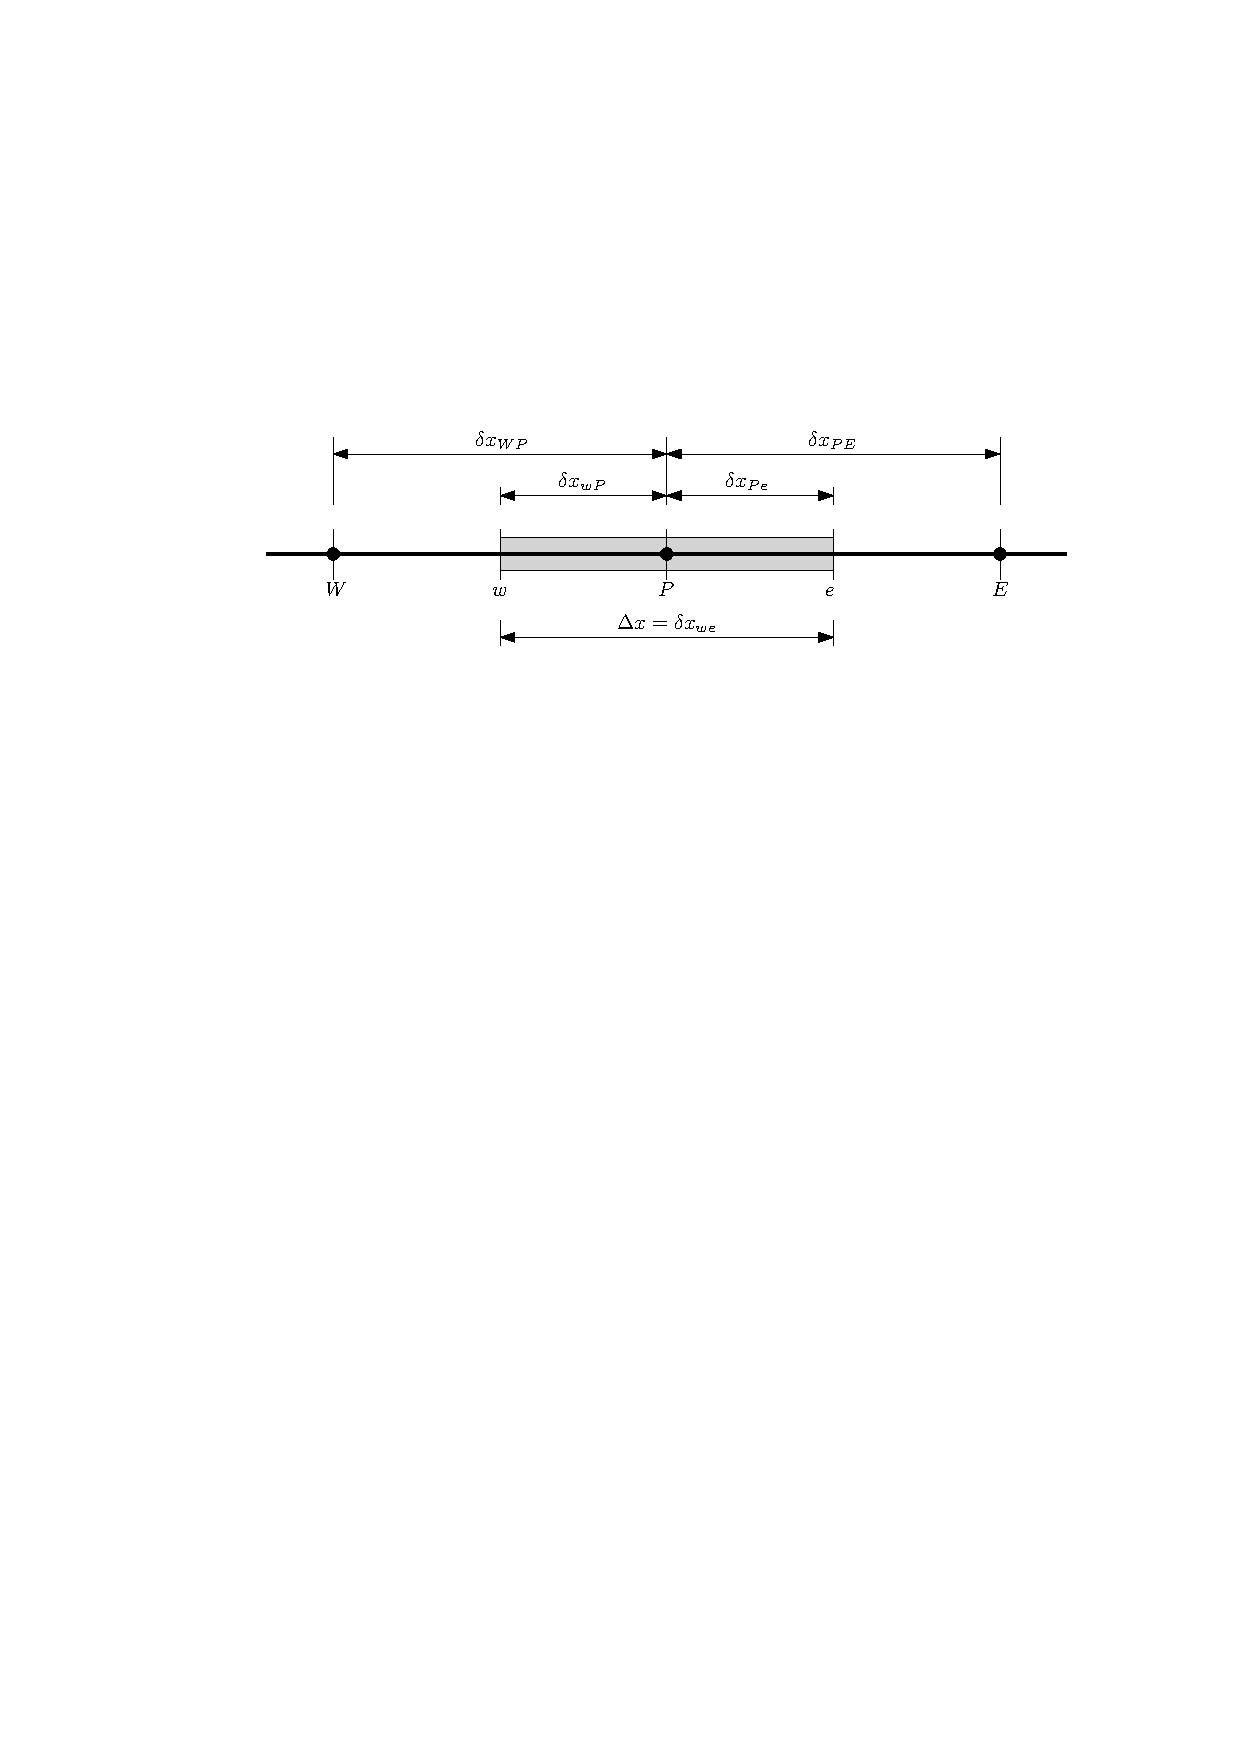
\includegraphics[width=0.8\textwidth]{FVmGridNotation.pdf}
\end{center}
\end{frame}

\begin{frame}{网格符号系统}
\begin{center}
  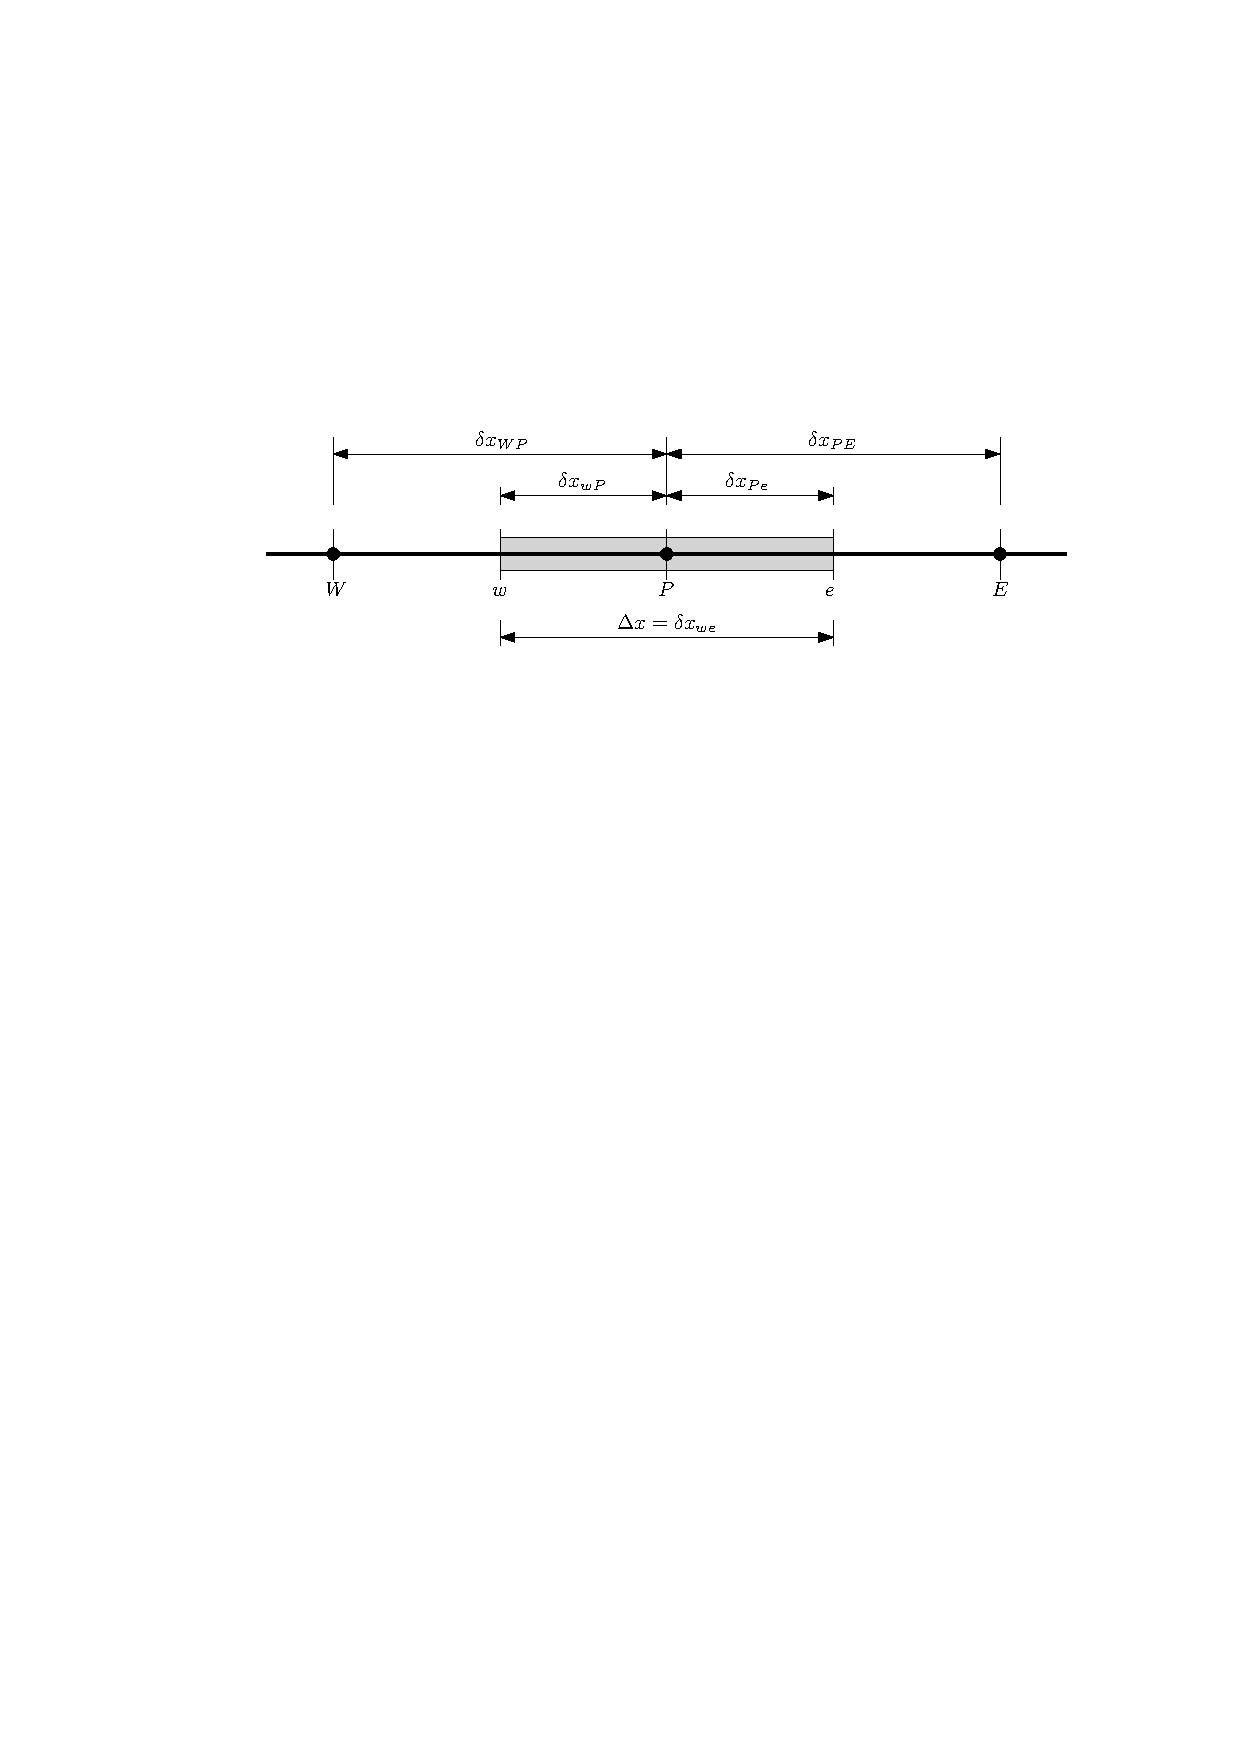
\includegraphics[width=0.8\textwidth]{FVmGridNotation.pdf}
\end{center}
  
\begin{itemize}
  \item $P$为网格系统中的任意节点,其西侧和东侧节点分别为$W$和$E$
  \item 节点$P$所在控制体西边的边界面为$w$,东边的边界面为$e$
  \item $W$与$P$的距离为$\delta x_{WP}$,$P$与$E$的距离为$\delta x_{PE}$
  \item $w$到$P$的距离为$\delta x_{wP}$,$P$到$e$的距离为$\delta x_{Pe}$
  \item $w$到$e$的距离为$\delta x_{we}$
\end{itemize}
\end{frame}

\subsection{步骤二:离散}
\begin{frame}{离散过程}
 \begin{description}
   \item[基本思想] 在控制体上对控制方程积分来得到控制体节点$P$上的离散方程
   \item[物理意义] 流出东边交界面的$\phi$的扩散通量减去流入西边交界面的$\phi$的扩散通量等于$\phi$的减少量
 \end{description} 
\begin{center}
  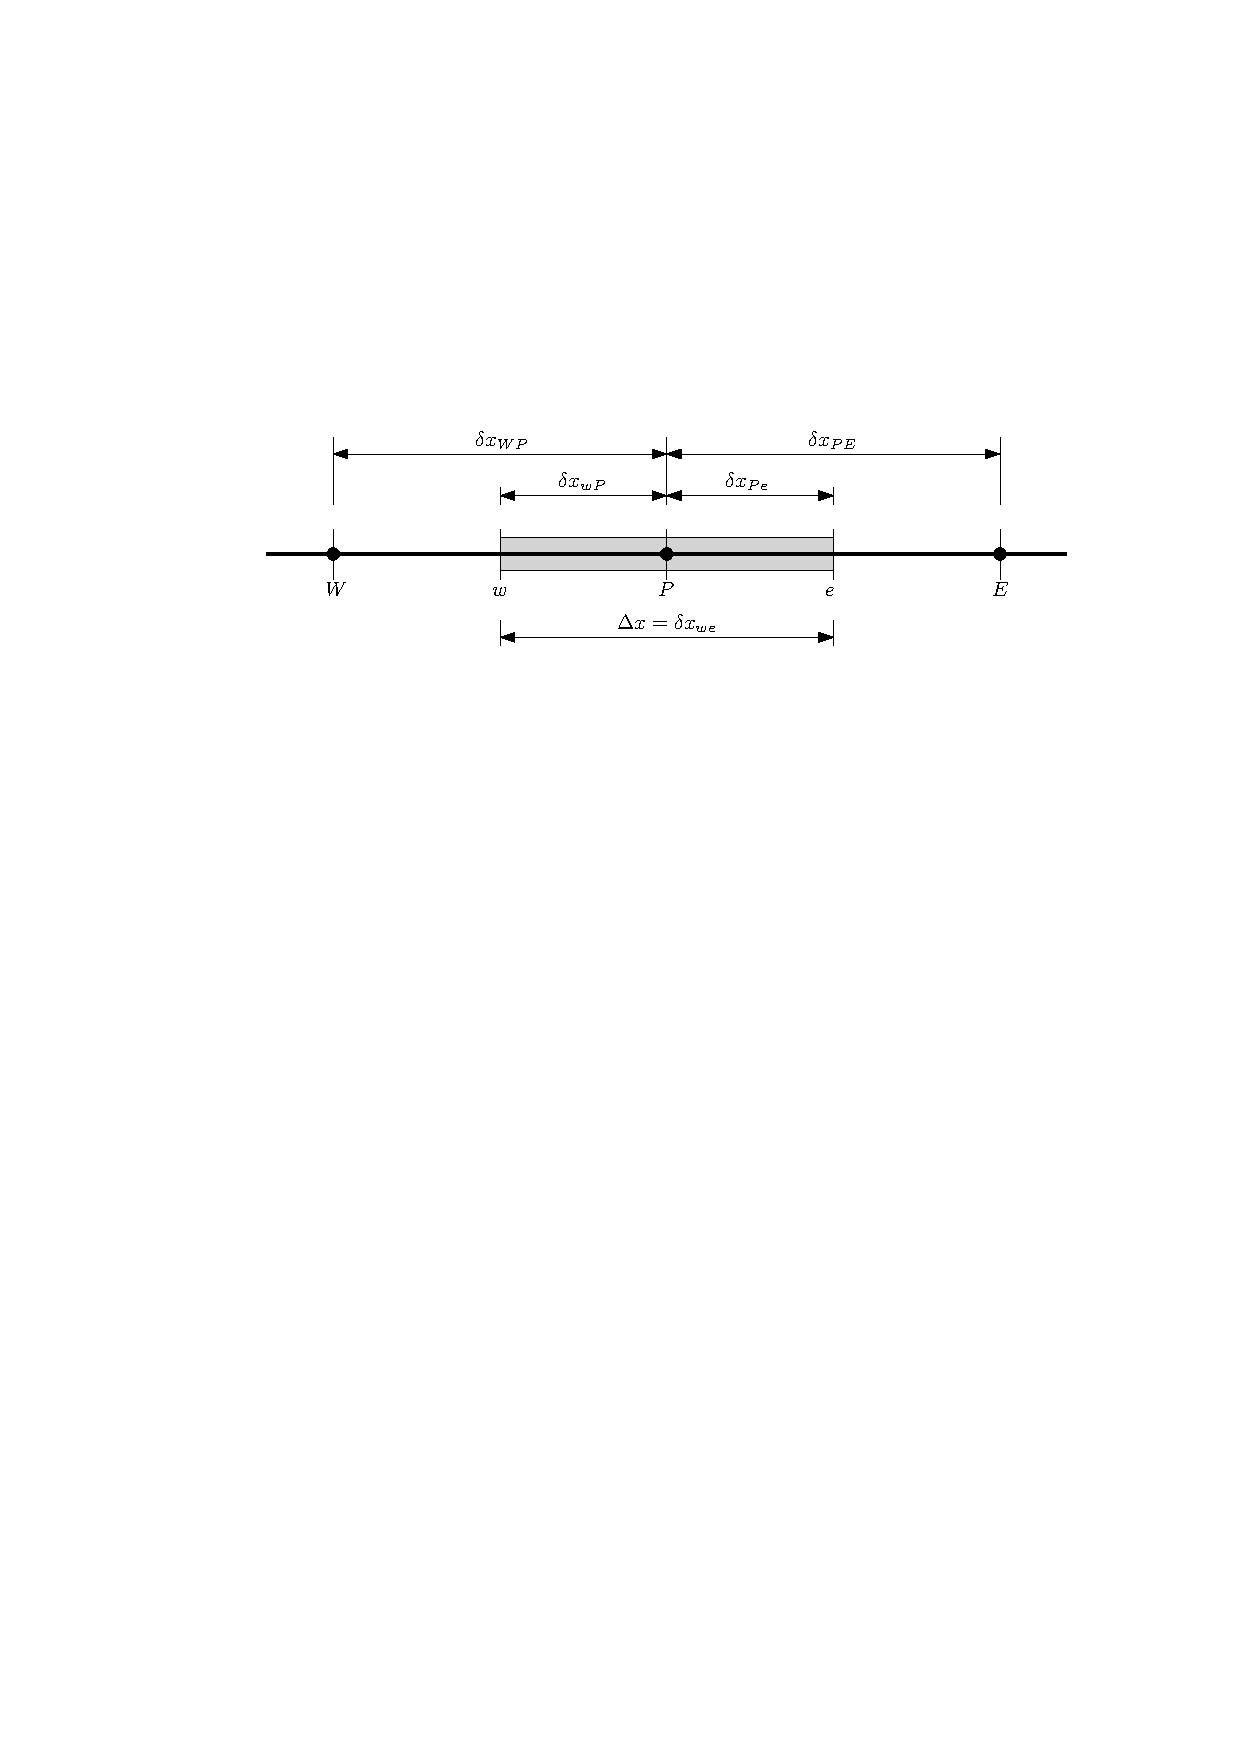
\includegraphics[width=0.7\textwidth]{FVmGridNotation.pdf}
\end{center}
\begin{equation*}
  \int_{\Delta V}\!
  \frac{\mathrm{d} }{\mathrm{d} x}
  \left(
    \Gamma \frac{\mathrm{d} \phi}{\mathrm{d} x}
  \right)
  \mathrm{d}V
  +
  \int_{\Delta V}\!
  S
  \mathrm{d}V
  =
  \left(
    \Gamma A\frac{\mathrm{d} \phi}{\mathrm{d} x}
  \right)_{e}
  -
  \left(
    \Gamma A\frac{\mathrm{d} \phi}{\mathrm{d} x}
  \right)_{w}
  +
  \overline{S}\Delta V
  =
  0
  \label{EqFV_Diffusion_Discretisation}
\end{equation*}

$A$为控制体边界面面积,$\Delta V$为控制体体积,$\overline{S}$为控制体上
$S$的平均值
\end{frame}

\begin{frame}{交界面梯度计算}
\begin{equation*}
  \begin{aligned}
  \Gamma_{w} 
  &=
  \frac{\Gamma_{W}+\Gamma_{P}}{2}
  \\
  \Gamma_{e} 
  &=
  \frac{\Gamma_{P}+\Gamma_{E}}{2}
  \end{aligned}
\end{equation*}
\begin{equation*}
  \begin{aligned}
  &\left(
    \Gamma A\frac{\mathrm{d} \phi}{\mathrm{d} x}
  \right)_{e}
  =
  \Gamma_{e}A_{e}
  \left(
    \frac{\phi_{E}-\phi_{P}}{\delta x_{PE}}
  \right)
    \\
  &\left(
    \Gamma A\frac{\mathrm{d} \phi}{\mathrm{d} x}
  \right)_{w}
  =
  \Gamma_{w}A_{w}
  \left(
    \frac{\phi_{P}-\phi_{W}}{\delta x_{WP}}
  \right)
  \end{aligned}
\end{equation*}
\end{frame}
为了推导出可用的离散方程,式\eqref{EqFV_Diffusion_Discretisation}中控制体交界面上的
$\Gamma$和梯度$\mathrm{d}\phi/\mathrm{d}x$必须要先求得。
\begin{equation}
  \overline{S}\Delta V = S_{u} + S_{P}\phi_{P}
\end{equation}
\begin{equation}
  \Gamma_{e}A_{e}
  \left(
    \frac{\phi_{E}-\phi_{P}}{\delta x_{PE}}
  \right)
  -
  \Gamma_{w}A_{w}
  \left(
    \frac{\phi_{P}-\phi_{W}}{\delta x_{WP}}
  \right)
  +
  (S_{u} + S_{P}\phi_{P})
  =
  0
\end{equation}
\begin{equation}
  \left(
    \frac{\Gamma}{\delta x_{PE}}A_{e}
    +
    \frac{\Gamma}{\delta x_{WP}}A_{w}
    -
    S_{p}
  \right)
  \phi_{P}
  =
  \left(
    \frac{\Gamma_{w}}{\delta x_{WP}}A_{w}
  \right)\phi_{W}
  +
  \left(
    \frac{\Gamma_{e}}{\delta x_{PE}}A_{e}
  \right)\phi_{E}
  +
  S_{u}
\end{equation}
\begin{equation}
  a_{P}\phi_{P} = a_{W}\phi_{W} + a_{E}\phi_{E}+S_{u}
  \label{EqFV_1dsd_fvm}
\end{equation}
其中
\begin{table}[H]
  \begin{center}
  %\caption{雅可比迭代结果}
  \label{TbFV_diffusion_coefficient}
  \begin{tabular}{|c|c|c|}
    \hline
    $a_{W}$ & $a_{E}$ & $a_{P}$
    \\
    \hline
    \makecell*[c]{
    $\displaystyle \frac{\Gamma_{w}}{\delta x_{WP}}A_{w}$
  }
            &
    $\displaystyle \frac{\Gamma_{e}}{\delta x_{PE}}A_{e}$
            &
    $a_{W} + a_{E} - S_{P}$
    \\
    \hline
  \end{tabular}
  \end{center}
\end{table}

\subsection{步骤三、求解}
式\eqref{EqFV_1dsd_fvm}必须在所有控制体的节点上都列出才能求解。对于毗邻计算域边
界的控制体,式\eqref{EqFV_1dsd_fvm}必须经过适当修正以包含边界条件。最后形成的线
性代数方程组可以通过上一章的求解方法来进行求解得到$\phi$的分布。

